%% ============================================================================
%%  NeuroAgent / NeuroBench -- Clinical collaboration proposal deck
%%  CERN beamer theme (cafein team variant + author-year citations)
%%
%%  Build: latexmk -pdf collab_prop.tex   (or via omnilib_compile_latex)
%%  Figures live in ./figures (regenerate with: make figures)
%%  Theme + logos: ./beamerthemeCERN.sty + ./logos/
%%
%%  Audience: prospective clinical partner / hospital (validators + co-authors)
%%  Status:   scaffold only -- content to be built step by step.
%% ============================================================================

%% `table' option for xcolor must reach xcolor BEFORE beamer loads it.
\PassOptionsToPackage{table}{xcolor}

%% `t' = top-align frame bodies; matches the CERN frametitle template.
\documentclass[aspectratio=169,t]{beamer}

%% [cafein]     -> auto-wires the CAFEIN logo + appends cafein.web.cern.ch
%% [authoryear] -> citations rendered as "Protani et al. (2024)" via natbib
\usetheme[authoryear]{CERN}

%% --- Extra packages (theme already loads tikz, graphicx, booktabs, colortbl)
\usepackage{pgfplots}
\pgfplotsset{compat=1.18}
\usepackage{listings}
\usepackage{array}
\usepackage{fontawesome5}
\usepackage{amsmath}
\usetikzlibrary{arrows.meta,positioning,calc,fit}

\lstset{
  basicstyle=\ttfamily\scriptsize,
  breaklines=true,
  showstringspaces=false,
  columns=fullflexible,
  keepspaces=true,
}

\graphicspath{{figures/}{figures/first_stage_review/}{logos/}}

%% ----------------------------------------------------------------------------
%% Custom placeholder commands -- replace with real assets later.
%%  \aiplaceholder[width]{prompt-idea}   for AI-generated hero images
%%  \screenshotph[width]{caption}        for product screenshots
%% ----------------------------------------------------------------------------
\newcommand{\aiplaceholder}[2][\linewidth]{%
  \begin{tikzpicture}
    \node[draw=CERNorange, very thick, dash pattern=on 4pt off 2pt,
          rounded corners=4mm, fill=CERNorange!7,
          inner sep=2mm, align=center,
          minimum height=34mm] {%
      \parbox{\dimexpr#1-6mm\relax}{\centering
        {\bfseries\normalsize\color{CERNorange}AI HERO IMAGE}\\[0.5mm]
        {\scriptsize\itshape\color{CERNtextdark}#2}}%
    };
  \end{tikzpicture}%
}

\newcommand{\screenshotph}[2][\linewidth]{%
  \begin{tikzpicture}
    \node[draw=CERNnavy, very thick,
          rounded corners=2mm, fill=CERNlightbg,
          inner sep=2mm, align=center,
          minimum height=34mm] {%
      \parbox{\dimexpr#1-6mm\relax}{\centering
        {\bfseries\normalsize\color{CERNnavy}APP SCREENSHOT}\\[0.5mm]
        {\scriptsize\itshape\color{CERNtextdark}#2}}%
    };
  \end{tikzpicture}%
}

% Full-page screenshot placeholder (fills the entire slide, no title/footer)
\newcommand{\screenshotpage}[1]{%
  \begin{tikzpicture}[remember picture, overlay]
    \node[draw=CERNnavy, very thick, rounded corners=3mm, fill=CERNlightbg,
          inner sep=6mm, align=center,
          minimum width=\paperwidth, minimum height=\paperheight]
      at (current page.center) {%
      \parbox{0.85\paperwidth}{\centering
        {\bfseries\Large\color{CERNnavy}APP SCREENSHOT}\\[3mm]
        {\footnotesize\itshape\color{CERNtextdark}#1}}%
    };
  \end{tikzpicture}%
}

%% ----------------------------------------------------------------------------
%% Deck metadata
%% ----------------------------------------------------------------------------
\title{NeuroAgent}
\subtitle{Building and validating an evidence-driven neurological Agentic System}
\author{Andrea Protani}
\date{\today}

\shortauthor{Andrea Protani}
\shorttitle{NeuroAgent -- PhD project update}
\event{PhD project update}

%% Pin the section list so the timeline is correct on first compile.
%% TODO: revise sections as we build the proposal narrative together.
\cernsections{Motivation, Dataset, Agent, Collaboration, Supervision, Outlook}

\begin{document}

%% ===========================================================================
%% Cover
%% ===========================================================================
\maketitle

%% ===========================================================================
%% Motivation: Q&A is not enough -> a new paradigm
%% ===========================================================================
\section{Motivation}

\begin{frame}{A new way of testing medical AI}
  \centering\footnotesize\color{CERNtextdark}
  Most research today tests medical AI with \alert{question answering}.
  Real clinical work is not like that.

  \vspace{2mm}
  \begin{columns}[T,onlytextwidth]
    \begin{column}{0.48\textwidth}
      \begin{block}{\faListOl\;\, Today: question answering}
        \footnotesize
        \begin{itemize}\setlength\itemsep{0.3em}
          \item Multiple-choice exams
          \item Every clue is already in the question
          \item One correct option to pick
          \item Rewards recall, not reasoning
        \end{itemize}
      \end{block}
    \end{column}%
    \hfill
    \begin{column}{0.48\textwidth}
      \begin{alertblock}{\faUserInjured\;\, Real clinical practice}
        \footnotesize
        \begin{itemize}\setlength\itemsep{0.3em}
          \item The patient arrives with a complaint, not options
          \item You decide which investigations to order
          \item Results come back over time
          \item Cost, risk and safety all matter
        \end{itemize}
      \end{alertblock}
    \end{column}
  \end{columns}

  \vspace{2mm}
  \begin{center}
  \begin{tikzpicture}
    \node[rounded corners=2mm, draw=CERNorange, line width=0.8pt,
          fill=CERNorange!10, inner sep=2.2mm,
          text width=0.9\textwidth, align=center]
    {\footnotesize\color{CERNtextdark}
      We introduce a \textbf{new paradigm}: test the AI on the
      \alert{whole diagnostic workup}, the way a clinician actually reasons.};
  \end{tikzpicture}
  \end{center}
\end{frame}

%% ===========================================================================
%% Project overview
%% ===========================================================================
\begin{frame}{Project overview}

  %% --- Step-by-step diagram: reason, test, revise -------------------------
  \begin{center}
  \begin{tikzpicture}[
    every node/.style={font=\scriptsize\sffamily, align=center},
    stage/.style={rectangle, rounded corners=2mm, very thick,
                  minimum width=20mm, minimum height=10mm,
                  align=center, inner sep=1mm},
    arr/.style={-{Stealth[length=2.2mm,width=2mm]}, very thick, CERNblue},
    larr/.style={-{Stealth[length=2.2mm,width=2mm]}, thick, dashed, CERNorange},
  ]
    \node[stage, draw=CERNnavy,   fill=CERNnavy!12]   (s1) at (0,0)
      {{\color{CERNnavy}\faUserInjured}\\\textbf{Initial}\\picture};
    \node[stage, draw=CERNblue,   fill=CERNblue!15]   (s2) at (2.9,0)
      {{\color{CERNblue}\faLightbulb}\\\textbf{Reason}\\hypothesis};
    \node[stage, draw=CERNorange, fill=CERNorange!18] (s3) at (5.8,0)
      {{\color{CERNorange}\faVial}\\\textbf{Order}\\one test};
    \node[stage, draw=CERNcyan,   fill=CERNcyan!22]   (s4) at (8.7,0)
      {{\color{CERNnavy}\faClipboardCheck}\\\textbf{Read}\\the result};
    \node[stage, draw=CERNblue,   fill=CERNblue!22]   (s5) at (11.6,0)
      {{\color{CERNblue}\faStethoscope}\\\textbf{Diagnosis}\\+ plan};

    \draw[arr] (s1) -- (s2);
    \draw[arr] (s2) -- (s3);
    \draw[arr] (s3) -- (s4);
    \draw[arr] (s4) -- (s5);
    \coordinate (lo1) at ($(s4.south)+(0,-0.34)$);
    \coordinate (lo2) at ($(s2.south)+(0,-0.34)$);
    \draw[larr, rounded corners=4pt] (s4.south) -- (lo1) -- (lo2) -- (s2.south);
    \node[font=\tiny\itshape, text=CERNorange, below=0pt]
      at ($(lo1)!0.5!(lo2)$) {revise and repeat, up to 15 steps};
  \end{tikzpicture}
  \end{center}

  \vspace{1.5mm}
  \centering\footnotesize
  \textbf{600 realistic neurology cases} across 20 conditions.

  \vspace{1.5mm}

  %% --- Two cards: what we score, why it is new -----------------------------
  \begin{columns}[T,onlytextwidth]
    \begin{column}{0.48\textwidth}
      \begin{block}{\faBullseye\;\, What we measure}
        \footnotesize
        \begin{itemize}\setlength\itemsep{0.3em}
          \item Right test, right order, sensible cost
          \item Sound reasoning, not memorised facts
          \item A workup a clinician can follow
        \end{itemize}
      \end{block}
    \end{column}%
    \hfill
    \begin{column}{0.48\textwidth}
      \begin{alertblock}{\faLightbulb\;\, Why it is new}
        \footnotesize
        \begin{itemize}\setlength\itemsep{0.3em}
          \item Today's AI exams hand over every clue
          \item Tests the real skill: what to investigate
          \item Each case checked by \textbf{2+ clinicians}
        \end{itemize}
      \end{alertblock}
    \end{column}
  \end{columns}
\end{frame}

%% ===========================================================================
%% The agent in action (screenshot): the goal
%% ===========================================================================
\begin{frame}{The agent in action}
  \centering\footnotesize\color{CERNtextdark}
  The goal: a transparent workup, ending in a diagnosis backed by evidence.

  \vspace{2mm}
  \tikz\node[draw=CERNnavy!35, line width=0.4pt, rounded corners=1mm,
             inner sep=0]{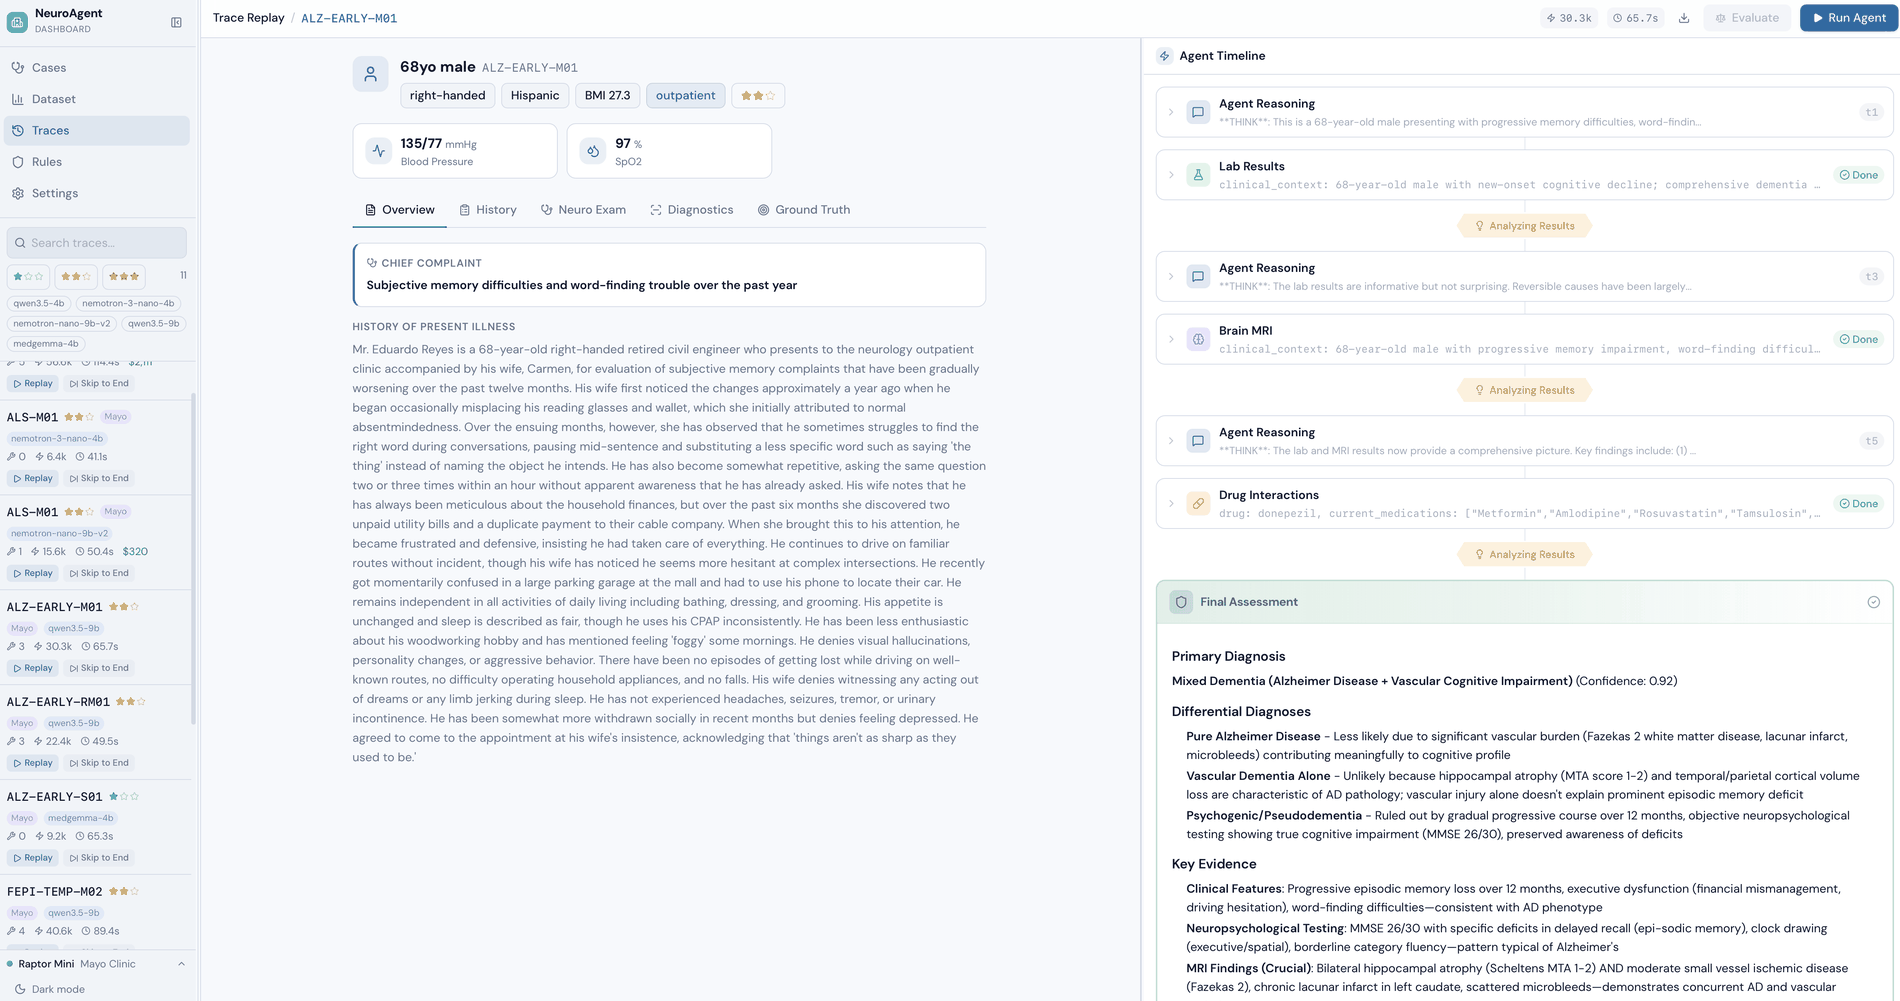
\includegraphics[height=5.5cm]{agent-in-action.png}};
\end{frame}

%% ===========================================================================
%% The dataset
%% ===========================================================================
\section{Dataset}

\begin{frame}{The dataset}
  \begin{columns}[T,onlytextwidth]
    \begin{column}{0.31\textwidth}
      \begin{block}{\faLayerGroup\;\, Cases}
        \centering
        \cernstatnum{600}

        \vspace{0.3mm}
        {\footnotesize 20 conditions}
      \end{block}
    \end{column}%
    \hfill
    \begin{column}{0.31\textwidth}
      \begin{alertblock}{\faBalanceScale\;\, Per condition}
        \centering
        \cernstatnum[CERNorange]{30}

        \vspace{0.3mm}
        {\footnotesize exactly, fully balanced}
      \end{alertblock}
    \end{column}%
    \hfill
    \begin{column}{0.31\textwidth}
      \begin{exampleblock}{\faDatabase\;\, Follow-up results}
        \centering
        \cernstatnum[CERNcyan]{3{,}800}

        \vspace{0.3mm}
        {\footnotesize triggered by actions}
      \end{exampleblock}
    \end{column}
  \end{columns}

  \vspace{1mm}
  \begin{columns}[T,onlytextwidth]
    \begin{column}{0.48\textwidth}
      \begin{block}{\faSitemap\;\, How each case is built}
        \footnotesize
        \begin{itemize}\setlength\itemsep{0.2em}
          \item Patient core: history, exam, vitals
          \item Evidence hidden behind tool calls
          \item Ground truth: best path, red herrings, unsafe actions
        \end{itemize}
      \end{block}
    \end{column}%
    \hfill
    \begin{column}{0.48\textwidth}
      \begin{alertblock}{\faThLarge\;\, Spanning}
        \footnotesize
        \begin{itemize}\setlength\itemsep{0.2em}
          \item 3 difficulty tiers: straightforward to puzzle
          \item 396 synthetic + 204 real-report-seeded
          \item 3 settings: emergency / inpatient / outpatient
        \end{itemize}
      \end{alertblock}
    \end{column}
  \end{columns}

  \vspace{1mm}
  \centering\scriptsize\itshape\color{CERNtextdark}
  Results are cached in two tiers: \textbf{initial} findings when a test is
  first ordered, and \textbf{follow-ups} unlocked by a specific next action.
\end{frame}

%% ===========================================================================
%% How the cases were generated
%% ===========================================================================
\begin{frame}{How the cases were generated}
  \centering\footnotesize\color{CERNtextdark}
  Two pipelines, one schema: real cases for fidelity, synthetic cases for scale.

  \vspace{1.5mm}
  \begin{columns}[T,onlytextwidth]
    \begin{column}{0.49\textwidth}
      \begin{block}{\faBookMedical\;\, Seeded from real case reports}
        \footnotesize
        \begin{itemize}\setlength\itemsep{0.25em}
          \item Source: \textbf{MedCaseReasoning}, clinician-written case reports
          \item Rewritten by \textbf{Claude Opus 4.8 + Sonnet 4.6}: findings
                hidden in tool outputs
        \end{itemize}
        \centering{\color{CERNblue}\bfseries 204 cases}
      \end{block}
    \end{column}%
    \hfill
    \begin{column}{0.49\textwidth}
      \begin{alertblock}{\faRobot\;\, Fully synthetic, for scale}
        \footnotesize
        \begin{itemize}\setlength\itemsep{0.25em}
          \item Built from per-condition clinical schemas, no source report
          \item Scale needed to \textbf{fine-tune local models}
          \item Same schema and ground truth as the seeded cases
        \end{itemize}
        \centering{\color{CERNorange}\bfseries 396 cases}
      \end{alertblock}
    \end{column}
  \end{columns}

\end{frame}

%% ===========================================================================
%% The 12 tools
%% ===========================================================================
\begin{frame}{The 12 diagnostic tools}
  \scriptsize
  \begin{cerntable}{@{}p{0.30\textwidth} p{0.62\textwidth}@{}}
    \cernheaderrow
    \cernth{Tool}               & \cernth{What it returns}                              \\
    Brain MRI                   & report with region-tagged findings                   \\
    EEG                         & background, epileptiform features, focality          \\
    ECG                         & rhythm, intervals, signs of ischaemia                \\
    Labs                        & panels with reference ranges + abnormality flags     \\
    CSF (lumbar puncture)       & cells, protein, glucose, NfL, oligoclonal bands       \\
    CT scan                     & non-contrast / contrast, head / spine                \\
    Echocardiogram              & chambers, valves, ejection fraction, thrombus        \\
    Cardiac monitoring          & telemetry / Holter / loop recorder                   \\
    Advanced imaging            & MRA / MRV / CTA / PET / DaT-SPECT                    \\
    Specialised tests           & EMG/NCS, biopsy, autoimmune panels                   \\
    Literature search           & guideline and paper snippets                          \\
    Drug interactions           & interaction profile + contraindications              \\
  \end{cerntable}

  \vspace{0.5mm}
  \centering\scriptsize\itshape\color{CERNtextdark}
  Each returns a structured, typed report with a cost; any tool, any time.
\end{frame}

%% ===========================================================================
%% Mechanism: every patient is a complete picture
%% ===========================================================================
\begin{frame}{Every patient is a complete picture}
  \centering\footnotesize\color{CERNtextdark}
  Each case pre-computes a \alert{whole patient}, so the agent can order
  \textbf{any} of the 12 tools and always get a realistic answer.

  \vspace{1mm}
  \begin{center}
  \begin{tikzpicture}[
    every node/.style={font=\scriptsize\sffamily, align=center},
    box/.style={rectangle, rounded corners=2mm, very thick, inner sep=2mm,
                align=center},
    arr/.style={-{Stealth[length=2.4mm,width=2mm]}, very thick, CERNblue},
  ]
    \node[box, draw=CERNblue, fill=CERNblue!10, text width=25mm, minimum height=15mm]
      (pat) at (0,0) {{\color{CERNblue}\faUserInjured}\\\textbf{Patient}\\history, exam,\\vitals};
    \node[box, draw=CERNnavy, fill=CERNnavy!10, text width=22mm, minimum height=15mm]
      (tools) at (3.9,0) {{\color{CERNnavy}\faToolbox}\\\textbf{Any of the}\\\textbf{12 tools}};
    \node[box, draw=CERNorange, fill=CERNorange!12, text width=46mm]
      (r1) at (9.1,1.0)
      {{\color{CERNorange}\faCheckCircle}\;\textbf{On the right pathway}\\the real finding that drives the diagnosis};
    \node[box, draw=CERNcyan, fill=CERNcyan!16, text width=46mm]
      (r2) at (9.1,-1.0)
      {{\color{CERNnavy}\faMinusCircle}\;\textbf{Off pathway}\\a realistic normal or incidental result};
    \draw[arr] (pat) -- (tools);
    \draw[arr] (tools.east) -- (r1.west);
    \draw[arr] (tools.east) -- (r2.west);
  \end{tikzpicture}
  \end{center}

  \vspace{1.5mm}
  \begin{center}
  \begin{tikzpicture}
    \node[rounded corners=2mm, draw=CERNorange, line width=0.8pt, fill=CERNorange!10,
          inner sep=2.2mm, text width=0.9\textwidth, align=center]
    {\footnotesize\color{CERNtextdark}
      \textbf{Never a dead end:} every tool answers. But each call costs money
      and a turn, so ordering the wrong test is \alert{penalised}.};
  \end{tikzpicture}
  \end{center}
\end{frame}

%% ===========================================================================
%% Worked example: ISCH-STR-M02 (wake-up stroke)
%% ===========================================================================
\begin{frame}{A worked example: wake-up ischemic stroke}
  \begin{columns}[T,onlytextwidth]
    \begin{column}{0.48\textwidth}
      \begin{block}{\faUserInjured\;\, Turn 1: what the agent sees}
        \footnotesize
        \begin{itemize}\setlength\itemsep{0.15em}
          \item 58\,F: woke with slurred speech, clumsy hand
          \item Last known well 9\,h ago: window unclear
          \item Left face/arm weak, sensory loss, neglect
        \end{itemize}
      \end{block}
    \end{column}%
    \hfill
    \begin{column}{0.48\textwidth}
      \begin{alertblock}{\faVial\;\, What the right workup reveals}
        \footnotesize
        \begin{itemize}\setlength\itemsep{0.15em}
          \item CT first: rule out bleed; glucose: no hypoglycemia
          \item MRI: fresh infarct, deep right white matter
          \item ECG, echo, carotids, Holter: hunt the cause
        \end{itemize}
      \end{alertblock}
    \end{column}
  \end{columns}

  \vspace{1mm}
  \begin{exampleblock}{\faMinusCircle\;\, The trap, and an off-pathway test}
    \footnotesize
    \alert{``Chronic, not acute''} tempts an early stop, yet the cause hunt is still owed. An off-pathway EEG reads \textbf{normal}: wasted.
  \end{exampleblock}

  \vspace{0.5mm}
  \centering\footnotesize\color{CERNnavy}
  {\faNotesMedical}\;\textbf{Ground truth:} acute ischemic stroke, right corona radiata (ICD-10 I63.541).
\end{frame}

%% ===========================================================================
%% Agentic system: architecture, early model results, and training path
%% ===========================================================================
\section{Agent}

\begin{frame}{Agent stack: from patient to judged trace}
  \vspace{-1mm}
  \begin{center}
  \begin{tikzpicture}[scale=0.84, transform shape,
    every node/.style={font=\scriptsize\sffamily, align=center},
    box/.style={rectangle, rounded corners=2mm, very thick,
                minimum width=22mm, minimum height=9mm,
                inner sep=1.2mm},
    smallbox/.style={box, text width=24mm, minimum width=27mm},
    arr/.style={-{Stealth[length=2.2mm,width=2mm]}, very thick, CERNblue},
    darr/.style={-{Stealth[length=2.2mm,width=2mm]}, thick, dashed, CERNorange},
  ]
    \node[box, draw=CERNnavy, fill=CERNnavy!10] (case) at (0,1.15)
      {{\color{CERNnavy}\faUserInjured}\\\textbf{Case}\\hidden workup};
    \node[box, draw=CERNblue, fill=CERNblue!12] (think) at (3,1.15)
      {{\color{CERNblue}\faLightbulb}\\\textbf{ReAct}\\thought};
    \node[box, draw=CERNorange, fill=CERNorange!14] (act) at (6,1.15)
      {{\color{CERNorange}\faToolbox}\\\textbf{Action}\\tool call};
    \node[box, draw=CERNcyan, fill=CERNcyan!18] (obs) at (9,1.15)
      {{\color{CERNnavy}\faClipboardCheck}\\\textbf{Observation}\\typed output};
    \node[box, draw=CERNblue, fill=CERNblue!18] (dx) at (12,1.15)
      {{\color{CERNblue}\faStethoscope}\\\textbf{Dx}\\plan};

    \node[smallbox, draw=CERNorange, fill=CERNorange!10] (tools) at (6,-0.65)
      {\textbf{12 tools}\\costed, typed};
    \node[smallbox, draw=CERNnavy, fill=CERNnavy!10] (cache) at (9,-0.65)
      {\textbf{Patient simulator}\\cached outputs};
    \node[smallbox, draw=CERNcyan, fill=CERNcyan!14] (trace) at (12,-0.65)
      {\textbf{Trace log}\\calls, costs, rationales};
    \node[smallbox, draw=CERNorange, fill=CERNorange!14] (judge) at (12,-2.15)
      {{\color{CERNorange}\faGavel}\;\textbf{Judge}\\8 reasoning scores};

    \draw[arr] (case) -- (think);
    \draw[arr] (think) -- (act);
    \draw[arr] (act) -- (obs);
    \draw[arr] (obs) -- (dx);
    \draw[arr] (act.south) -- (tools.north);
    \draw[arr] (tools.east) -- (cache.west);
    \draw[arr] (cache.north) -- (obs.south);
    \draw[arr] (dx.south) -- (trace.north);
    \draw[arr] (trace.south) -- (judge.north);
    \draw[darr, rounded corners=4pt]
      (obs.north) -- ++(0,0.58) -- ($(think.north)+(0,0.58)$) -- (think.north);
    \node[font=\tiny\itshape, text=CERNorange] at (6,2.12) {repeat up to 15 turns};
  \end{tikzpicture}
  \end{center}

  \vspace{-1mm}
  \begin{exampleblock}{\faDatabase\;\, Why this matters clinically}
    \scriptsize
    Every run is replayable: ordered tests, revealed evidence, cost/safety
    events, and an independent reasoning-judge score.
  \end{exampleblock}
\end{frame}

\begin{frame}{Preliminary base-model results}
  \scriptsize
  \centering
  \begin{cerntable}{@{}p{0.27\textwidth} r r r r r@{}}
    \cernheaderrow
    \cernth{Model} & \cernth{Composite} & \cernth{Top-1} & \cernth{Top-3} &
    \cernth{Tool F1} & \cernth{Safety fails} \\
    qwen3.5-9b           & 0.779 & 35.3\% & 63.3\% & 0.56 & 28/150 \\
    qwen3.5-4b           & 0.671 & 36.7\% & 48.7\% & 0.46 & 45/150 \\
    nemotron-nano-9b-v2  & 0.565 & 11.3\% & 24.0\% & 0.28 & 82/150 \\
    gemma-4-e2b          & 0.538 & 13.3\% & 33.3\% & 0.35 & 72/150 \\
    gemma-4-e4b          & 0.483 & 12.0\% & 19.3\% & 0.26 & 90/150 \\
    nemotron-3-nano-4b   & 0.339 &  5.3\% &  8.0\% & 0.06 & 130/150 \\
  \end{cerntable}

  \vspace{1mm}
  \begin{columns}[T,onlytextwidth]
    \begin{column}{0.49\textwidth}
      \begin{block}{\faChartLine\;\, What the pilot says}
        \scriptsize
        50 random v5 cases, 3 repeats per case and model: 900 ReAct traces
        judged by an independent LLM judge. Qwen3.5 leads on composite score
        and top-3 calibration.
      \end{block}
    \end{column}%
    \hfill
    \begin{column}{0.49\textwidth}
      \begin{alertblock}{\faExclamationTriangle\;\, Failure modes to validate}
        \scriptsize
        Lumbar puncture ordered before imaging, unsafe medication advice,
        text-only fake tool calls, and weak reasoning to positively diagnose
        functional neurological disorder recur across models.
      \end{alertblock}
    \end{column}
  \end{columns}
\end{frame}

\begin{frame}{What those metrics mean}
  \vspace{-1mm}
  \begin{columns}[T,onlytextwidth]
    \begin{column}{0.49\textwidth}
      \begin{block}{\faBullseye\;\, Rule-based checks}
        \scriptsize
        \begin{itemize}\setlength\itemsep{0.08em}
          \item \textbf{Top-1:} final diagnosis matches the ground-truth ICD group
          \item \textbf{Top-3:} correct ICD group appears anywhere in the differential
          \item \textbf{Tool F1:} called tools vs the optimal workup sequence
          \item \textbf{Safety fails:} contraindicated, harmful, or wrong-order actions
        \end{itemize}
      \end{block}
    \end{column}%
    \hfill
    \begin{column}{0.49\textwidth}
      \begin{alertblock}{\faGavel\;\, LLM-judge composite}
        \scriptsize
        \begin{itemize}\setlength\itemsep{0.08em}
          \item \textbf{Judge dims:} 8 clinical-reasoning scores, each 0--5
          \item \textbf{Composite:} weighted mean, normalised to 0--1
          \item \textbf{Main weights:} diagnosis accuracy + clinical safety
          \item \textbf{Also checks:} evidence use, differential, uncertainty,
                tool efficiency, red herrings
        \end{itemize}
      \end{alertblock}
    \end{column}
  \end{columns}

  \vspace{0.4mm}
  \centering\scriptsize\color{CERNtextdark}
  {\color{CERNcyan}\faUserMd}\;\textbf{Clinician validation:}
  cases and sampled runs, including field correctness, hypothesis quality,
  unsafe reasoning, and score/clinical-quality alignment.

  \vspace{0.3mm}
  {\tiny\itshape\color{CERNtextdark}ICD = International Classification of
  Diseases, the WHO standard diagnostic coding system used to check whether
  the model's diagnosis matches the ground truth.}
\end{frame}

\begin{frame}{Fine-tuning approach: SFT w golden trajectories}
  \vspace{-1mm}
  \begin{columns}[T,onlytextwidth]
    \begin{column}{0.53\textwidth}
      \begin{block}{\faRoute\;\, Supervised Fine Tuning corpus}
        \footnotesize
        \begin{enumerate}\setlength\itemsep{0.10em}
          \item \textbf{Input:} clinician-approved optimal action sequence
          \item \textbf{Trace:} rationale $\rightarrow$ tool call $\rightarrow$
                cached result $\rightarrow$ next rationale
          \item \textbf{Filter:} correct diagnosis, no unsafe / wrong-order actions
          \item \textbf{Lock:} train only on clinician-validated cases
        \end{enumerate}
      \end{block}
    \end{column}%
    \hfill
    \begin{column}{0.43\textwidth}
      \begin{exampleblock}{\faMicrochip\;\, LoRA / QLoRA}
        \scriptsize
        \textbf{LoRA:} adapters; base frozen\\[-0.1mm]
        \textbf{QLoRA:} 4-bit frozen base\\[-0.1mm]
        \textbf{Trainable:} 116.4M / 9.07B params (1.28\%)\\[-0.1mm]
        \textbf{Fits:} long ReAct traces on one A100-40\,GB\\[0.4mm]
        {\tiny\itshape Hybrid model: attention LoRA only on the 8/32
        full-attention layers; MLP LoRA on all 32.}
      \end{exampleblock}
      \begin{alertblock}{\faBalanceScale\;\, Why SFT is not enough}
        \scriptsize
        \textbf{Learns:} ideal path\\[-0.1mm]
        \textbf{Misses:} recovery after a wrong early test\\[-0.1mm]
        \textbf{Needs:} scored sampled trajectories
      \end{alertblock}
    \end{column}
  \end{columns}
\end{frame}

\begin{frame}{RL roadmap: optimise scored trajectories}
  \begin{columns}[T,onlytextwidth]
    \begin{column}{0.49\textwidth}
      \begin{block}{\faRandom\;\, GRPO \emph{(planned)}}
        \scriptsize
        \begin{itemize}\setlength\itemsep{0.03em}
          \item \textbf{Sample:} several workups for one case
          \item \textbf{Score:} benchmark each trajectory
          \item \textbf{Update:} improve vs group average
          \item \textbf{No value model}
        \end{itemize}
      \end{block}
    \end{column}%
    \hfill
    \begin{column}{0.49\textwidth}
      \begin{exampleblock}{\faSlidersH\;\, DAPO \emph{(planned)}}
        \scriptsize
        \begin{itemize}\setlength\itemsep{0.03em}
          \item \textbf{Target:} longer reasoning traces
          \item \textbf{Keep:} useful hard trajectories
          \item \textbf{Reduce:} noisy clipping effects
          \item \textbf{Focus:} updates where gains remain
        \end{itemize}
      \end{exampleblock}
    \end{column}
  \end{columns}

  \vspace{0.8mm}
  \begin{alertblock}{\faClipboardCheck\;\, Reward signal}
    \scriptsize
    \centering
    trajectory $\rightarrow$ benchmark scores $\rightarrow$ composite reward $\rightarrow$ policy update

    \vspace{0.3mm}
    \tiny
    diagnosis \;|\; evidence \;|\; tools/order \;|\; cost \;|\; contraindications \;|\; red herrings \;|\; uncertainty
  \end{alertblock}
\end{frame}

\begin{frame}{Hypothesis DAG: make reasoning inspectable}
  \vspace{-1mm}
  \begin{center}
  \begin{tikzpicture}[
    every node/.style={font=\scriptsize\sffamily, align=center},
    nodebox/.style={rectangle, rounded corners=2mm, very thick,
                    inner sep=1.5mm, minimum width=22mm, minimum height=8mm},
    reviewbox/.style={rectangle, rounded corners=2mm, very thick,
                      inner sep=1.4mm, minimum width=27mm, minimum height=8mm},
    arr/.style={-{Stealth[length=2.1mm,width=1.8mm]}, very thick, CERNblue},
    sys/.style={-{Stealth[length=2.1mm,width=1.8mm]}, thick, dashed, CERNorange},
  ]
    \node[nodebox, draw=CERNnavy, fill=CERNnavy!10] (f1) at (0,0.75)
      {{\color{CERNnavy}\faUserInjured}\\Finding};
    \node[nodebox, draw=CERNnavy, fill=CERNnavy!10] (f2) at (0,-0.75)
      {{\color{CERNnavy}\faClipboardList}\\Exam};
    \node[nodebox, draw=CERNblue, fill=CERNblue!12] (h1) at (2.9,0)
      {{\color{CERNblue}\faLightbulb}\\Hypothesis};
    \node[reviewbox, draw=CERNorange, fill=CERNorange!12] (rev) at (2.9,1.65)
      {{\color{CERNorange}\faRobot}\\Review subagent};
    \node[nodebox, draw=CERNorange, fill=CERNorange!12] (a1) at (5.7,0.75)
      {{\color{CERNorange}\faVial}\\Action};
    \node[nodebox, draw=CERNcyan, fill=CERNcyan!18] (e1) at (5.7,-0.75)
      {{\color{CERNnavy}\faClipboardCheck}\\Evidence};
    \node[nodebox, draw=CERNblue, fill=CERNblue!18] (c1) at (8.6,0)
      {{\color{CERNblue}\faStethoscope}\\Conclusion};

    \draw[arr] (f1.east) -- (h1.west);
    \draw[arr] (f2.east) -- (h1.west);
    \draw[arr] (h1.east) -- (a1.west);
    \draw[arr] (a1.south) -- (e1.north);
    \draw[arr] (e1.east) -- (c1.west);
    \draw[sys] (h1.north) -- node[right, font=\tiny, text=CERNorange]
      {auto review} (rev.south);
  \end{tikzpicture}
  \end{center}

  \vspace{-0.8mm}
  \begin{columns}[T,onlytextwidth]
    \begin{column}{0.49\textwidth}
      \begin{block}{\faSitemap\;\, Typed nodes}
        \scriptsize
        \textbf{Finding / exam:} observed facts\\[-0.2mm]
        \textbf{Hypothesis:} candidate diagnosis\\[-0.2mm]
        \textbf{Action / evidence:} test and result\\[-0.2mm]
        \textbf{Conclusion:} final diagnosis + plan
      \end{block}
    \end{column}%
    \hfill
    \begin{column}{0.49\textwidth}
      \begin{exampleblock}{\faProjectDiagram\;\, Typed edges}
        \scriptsize
        \texttt{supports}: adds weight\\[-0.2mm]
        \texttt{contradicts}: weakens a hypothesis\\[-0.2mm]
        \texttt{triggers}: justifies an action\\[-0.2mm]
        \texttt{depends-on}: records prerequisites
      \end{exampleblock}
    \end{column}
  \end{columns}
\end{frame}

\begin{frame}{System-triggered hypothesis review subagent}
  \vspace{-1.8mm}
  \begin{center}
  \begin{tikzpicture}[
    every node/.style={font=\scriptsize\sffamily, align=center},
    box/.style={rectangle, rounded corners=2mm, very thick, inner sep=1.5mm,
                minimum width=27mm, minimum height=8mm},
    arr/.style={-{Stealth[length=2.1mm,width=1.8mm]}, very thick, CERNblue},
    sarr/.style={-{Stealth[length=2.1mm,width=1.8mm]}, thick, dashed, CERNorange},
  ]
    \node[box, draw=CERNblue, fill=CERNblue!12] (h) at (0,0)
      {{\color{CERNblue}\faLightbulb}\\New hypothesis};
    \node[box, draw=CERNorange, fill=CERNorange!12] (r) at (3.6,0)
      {{\color{CERNorange}\faRobot}\\Reviewer};
    \node[box, draw=CERNcyan, fill=CERNcyan!18] (c) at (7.2,0)
      {{\color{CERNnavy}\faPen}\\Critique};
    \node[box, draw=CERNnavy, fill=CERNnavy!10] (d) at (10.8,0)
      {{\color{CERNnavy}\faProjectDiagram}\\DAG writeback};
    \draw[sarr] (h) -- node[above, font=\tiny, text=CERNorange] {automatic} (r);
    \draw[arr] (r) -- (c);
    \draw[arr] (c) -- (d);
  \end{tikzpicture}
  \end{center}

  \vspace{-0.4mm}
  \begin{columns}[T,onlytextwidth]
    \begin{column}{0.50\textwidth}
      \begin{block}{\faRobot\;\, Trigger rule}
        \scriptsize
        \textbf{When:} each new hypothesis node\\[-0.2mm]
        \textbf{Who:} system, not acting agent\\[-0.2mm]
        \textbf{Why:} critique cannot be skipped
      \end{block}
      \begin{alertblock}{\faSearch\;\, Review checklist}
        \scriptsize
        differentials \;|\; evidence gaps \;|\; contradictions\\[-0.2mm]
        premature closure \;|\; unsafe next actions\\[-0.2mm]
        test justification
      \end{alertblock}
    \end{column}%
    \hfill
    \begin{column}{0.47\textwidth}
      \begin{exampleblock}{\faPen\;\, Structured writeback}
        \scriptsize
        \texttt{severity} \;|\; \texttt{claim} \;|\; \texttt{evidence\_node}\\[-0.2mm]
        \texttt{recommended\_fix} \;|\; \texttt{clinician\_review\_needed}
      \end{exampleblock}
      \begin{block}{\faUserMd\;\, Clinician validation}
        \scriptsize
        cases + sampled runs\\[-0.2mm]
        hypothesis quality + unsafe reasoning\\[-0.2mm]
        clinical usefulness of DAG critiques
      \end{block}
    \end{column}
  \end{columns}
\end{frame}

%% ===========================================================================
%% What we are asking: the collaboration
%% ===========================================================================
\section{Collaboration}

\begin{frame}{Goals for the medical collaboration}
  \centering\footnotesize\color{CERNtextdark}
  \begin{columns}[T,onlytextwidth]
    \begin{column}{0.49\textwidth}
      \begin{block}{\faStethoscope\;\, 1.\ Validate the cases}
        \footnotesize
        \begin{itemize}\setlength\itemsep{0.2em}
          \item Read each patient as you would in clinic
          \item Approve, flag, or correct field by field
          \item Drop cases that are not good enough
        \end{itemize}
      \end{block}
    \end{column}%
    \hfill
    \begin{column}{0.49\textwidth}
      \begin{alertblock}{\faGavel\;\, 2.\ Validate our scoring}
        \footnotesize
        \begin{itemize}\setlength\itemsep{0.2em}
          \item Score a sample of agent runs yourself
          \item Compare against the AI reasoning judge
          \item Confirm scores track clinical quality
        \end{itemize}
      \end{alertblock}
    \end{column}
  \end{columns}

  \vspace{1.5mm}
  \begin{exampleblock}{\faUsers\;\, How the review works}
    \footnotesize
    \begin{itemize}\setlength\itemsep{0.15em}
      \item $\geq$\textbf{2 independent reviewers} per case
      \item Separate login per reviewer: blind, no shared bias
      \item Agreement stats $\rightarrow$ fix or drop weak cases $\rightarrow$ higher quality
    \end{itemize}
  \end{exampleblock}
\end{frame}

%% ===========================================================================
%% The annotation platform (screenshots): browse + case view
%% ===========================================================================
\begin{frame}{The annotation platform}
  \begin{columns}[T,onlytextwidth]
    \begin{column}{0.49\textwidth}
      \centering
      \tikz\node[draw=CERNnavy!35, line width=0.4pt, rounded corners=1mm,
                 inner sep=0]{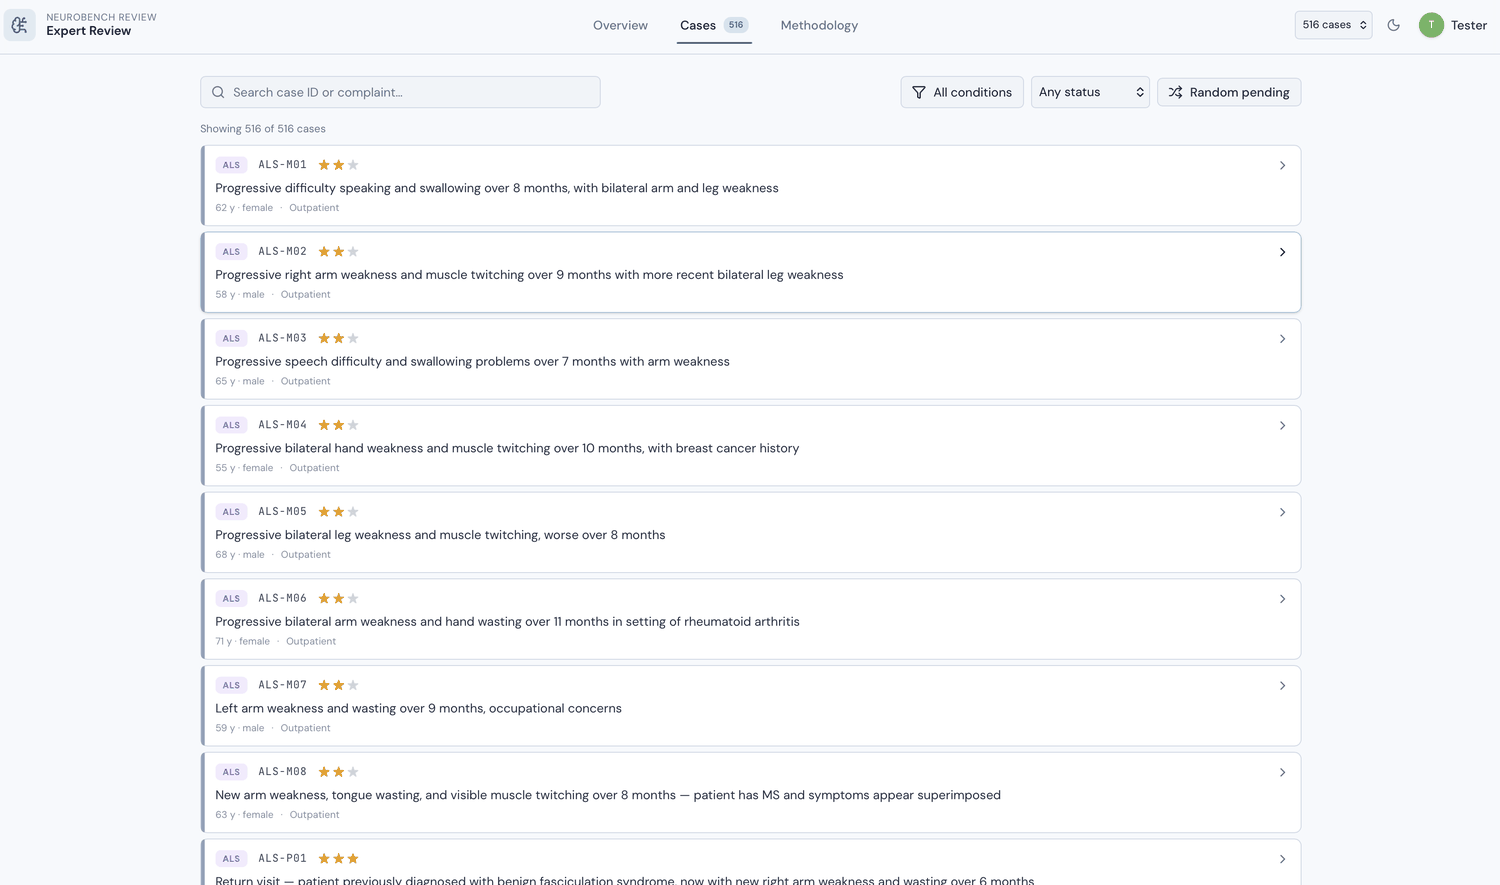
\includegraphics[height=4.0cm]{review-cases.png}};

      \vspace{0.8mm}
      {\scriptsize\color{CERNnavy}\faThList\;\, Browse cases: condition, difficulty, status}
    \end{column}%
    \hfill
    \begin{column}{0.49\textwidth}
      \centering
      \tikz\node[draw=CERNnavy!35, line width=0.4pt, rounded corners=1mm,
                 inner sep=0]{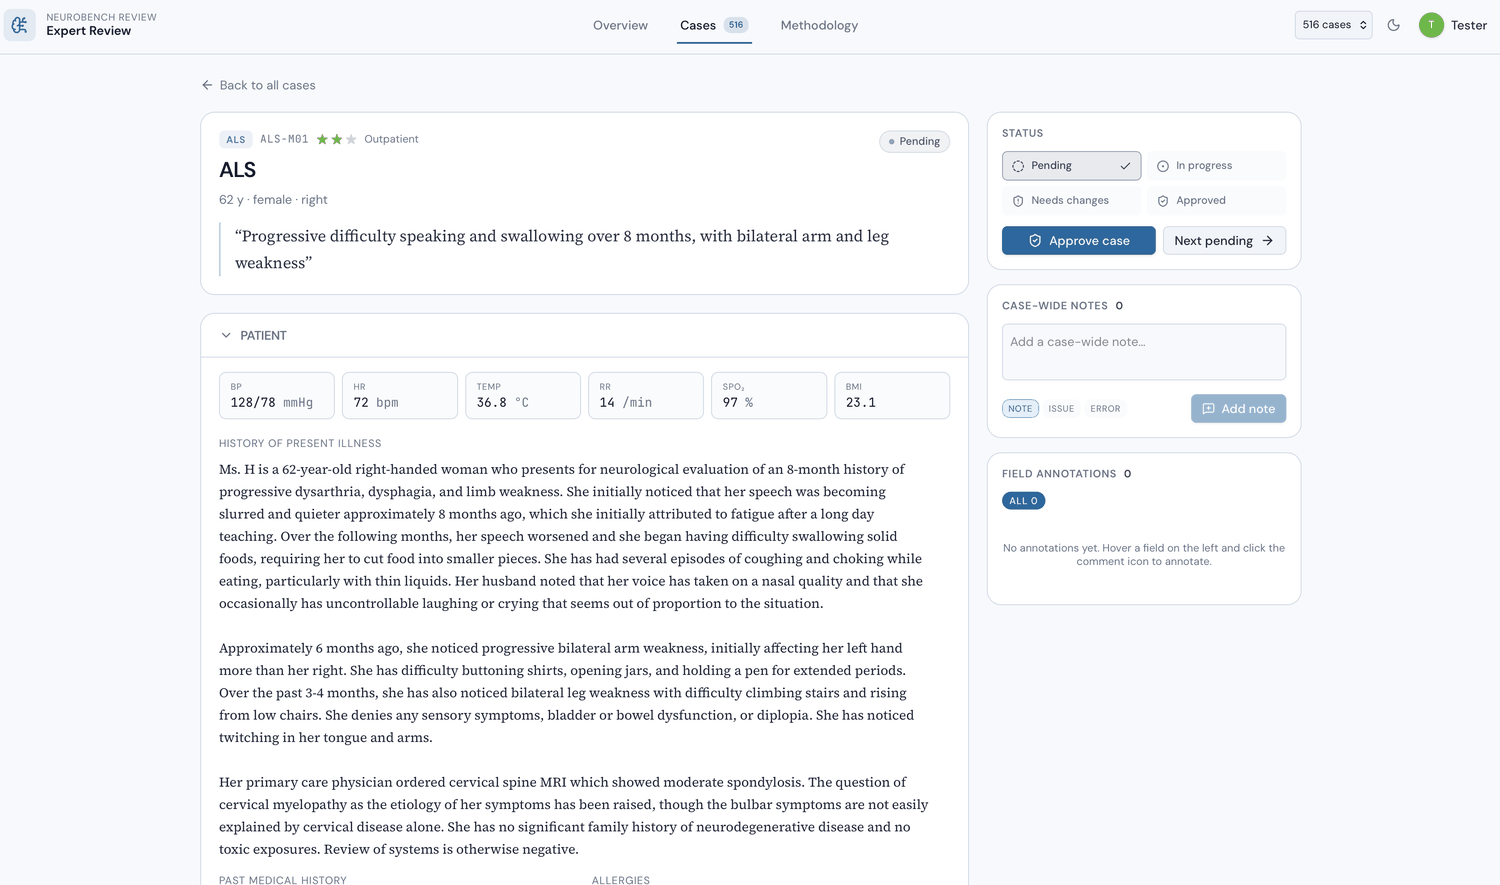
\includegraphics[height=4.0cm]{review-case.png}};

      \vspace{0.8mm}
      {\scriptsize\color{CERNnavy}\faUserInjured\;\, One screen per patient: vitals, history, full workup}
    \end{column}
  \end{columns}

  \vspace{3.5mm}
  \centering\footnotesize
  \faLink\;\,\href{https://review.andreaprotani.com}{\color{CERNblue}review.andreaprotani.com}

\end{frame}

%% ===========================================================================
%% Reviewing a case: annotate + status
%% ===========================================================================
\begin{frame}{Reviewing a case}
  \begin{columns}[T,onlytextwidth]
    \begin{column}{0.62\textwidth}
      \centering
      \tikz\node[draw=CERNnavy!35, line width=0.4pt, rounded corners=1mm,
                 inner sep=0]{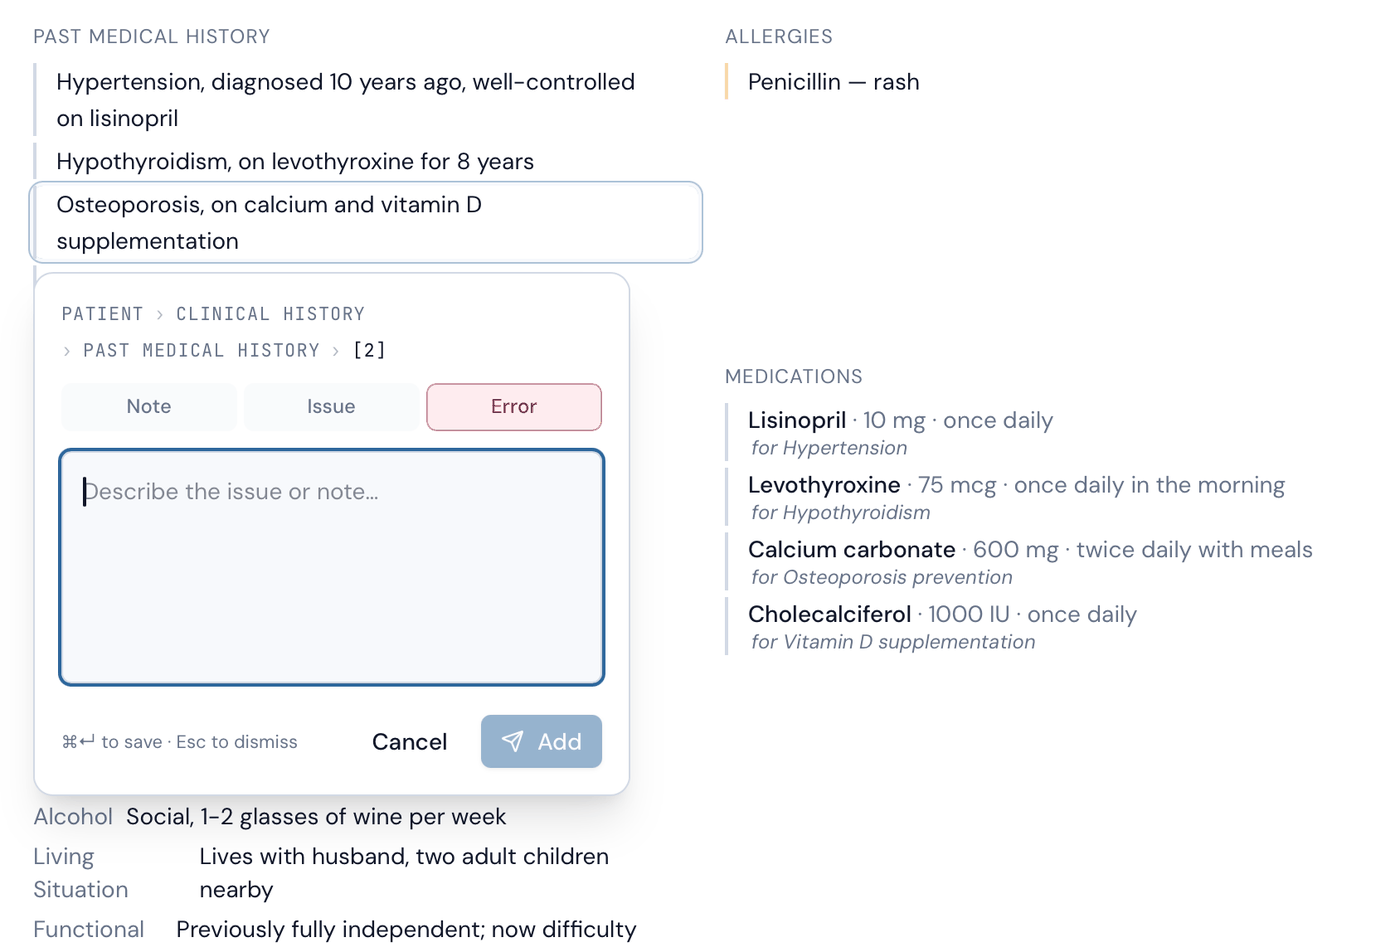
\includegraphics[height=4.3cm]{review-annotate.png}};

      \vspace{1.2mm}
      {\scriptsize\color{CERNnavy}\faCommentDots\;\, Flag any field: note, issue, or error}
    \end{column}%
    \hfill
    \begin{column}{0.36\textwidth}
      \centering
      \tikz\node[draw=CERNnavy!35, line width=0.4pt, rounded corners=1mm,
                 inner sep=0]{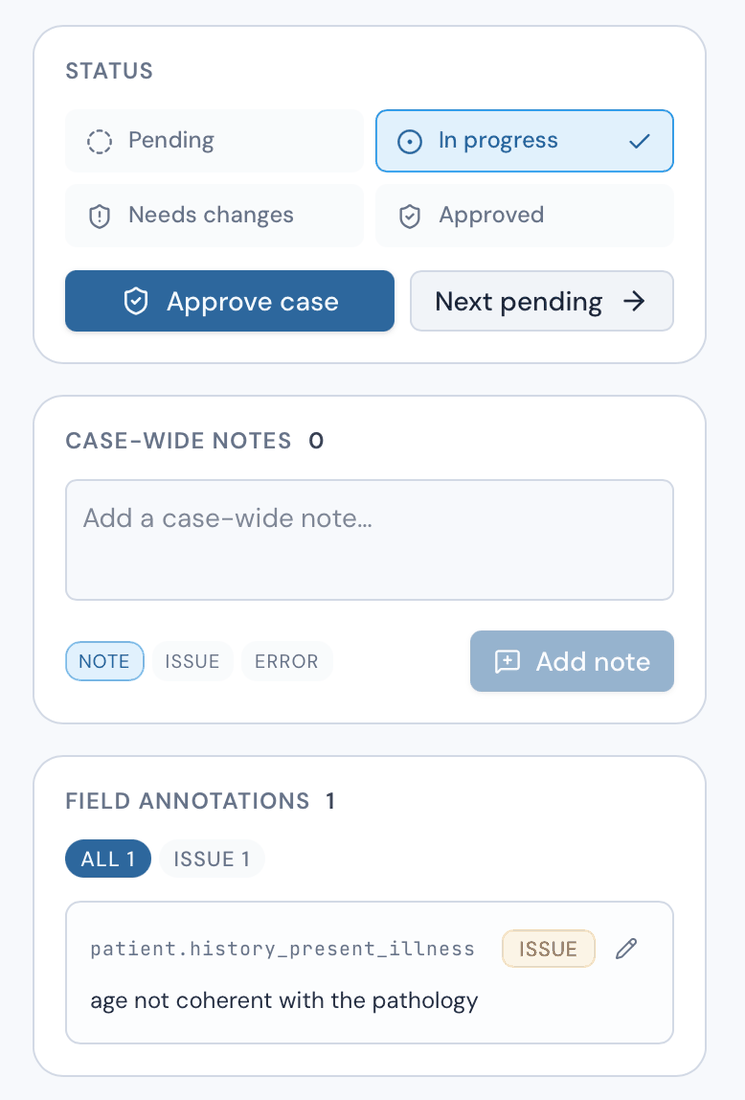
\includegraphics[height=4.3cm]{review-status.png}};

      \vspace{1.2mm}
      {\scriptsize\color{CERNnavy}\faTasks\;\, Per-case status, every annotation logged}
    \end{column}
  \end{columns}

  \vspace{2mm}
  \centering\scriptsize\itshape\color{CERNtextdark}
  Approve, request changes, or move on: progress tracked per reviewer.
\end{frame}

%% ===========================================================================
%% Outlook: related MSc supervision -- EEG source localisation
%% ===========================================================================
\section{Supervision}

\begin{frame}{Research objective}
  \centering\footnotesize\color{CERNtextdark}
  \textbf{Goal:} \alert{EEG source localization} $\rightarrow$ estimate a distribution over
  plausible cortical sources from EEG, while remaining \textbf{montage-agnostic}.

  \vspace{0.8mm}
  {\scriptsize\color{CERNnavy}\faUserGraduate\;\, Related MSc thesis project, supervised with \textbf{Lorenzo Sibi}
   \;\textbar\;\; \faLinkedin\;\,\href{https://www.linkedin.com/in/lorenzo-sibi/}{linkedin.com/in/lorenzo-sibi}}

  \vspace{1.3mm}
  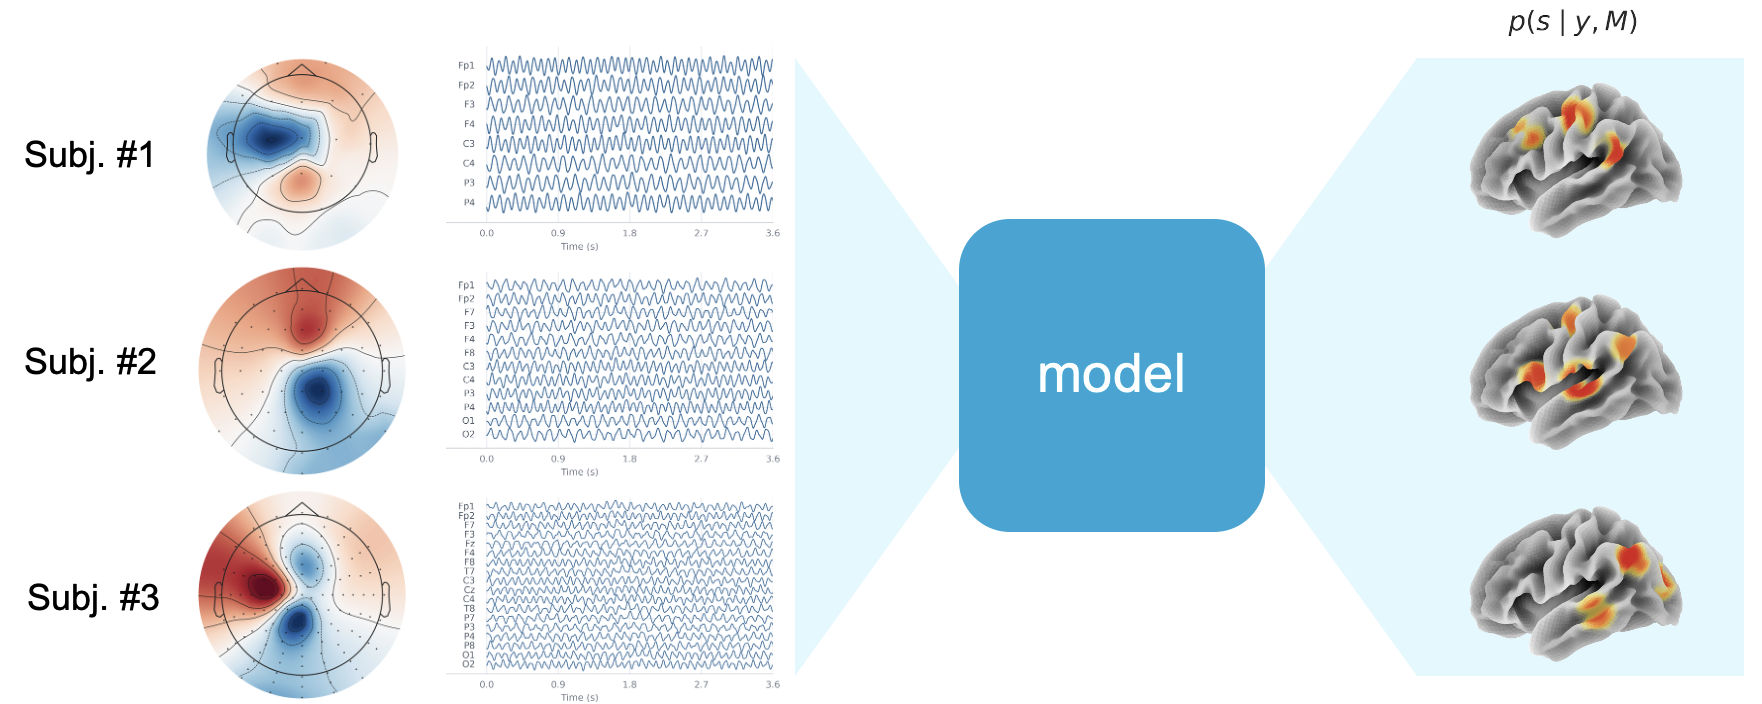
\includegraphics[height=40mm]{img1.png}

  \vspace{1.3mm}
  \footnotesize\color{CERNorange}
  The output should expose \textbf{uncertainty}: more than one source map can fit the same EEG.
\end{frame}

\begin{frame}{Synthetic dataset generation}
  \centering\footnotesize\color{CERNtextdark}
  Training needs many paired (EEG, source) samples; real ground truth needs intracerebral stimulation, which is rare.

  \vspace{0.3mm}
  \begin{tikzpicture}[
    every node/.style={font=\scriptsize\sffamily, align=center},
    arr/.style={-{Stealth[length=2.2mm,width=1.8mm]}, very thick, CERNblue},
    box/.style={rounded corners=2mm, line width=0.9pt, inner sep=1.1mm, minimum height=7mm},
  ]
    \node[box, draw=CERNnavy, fill=CERNnavy!10, text width=22mm] (sereega) at (-5.3,0.48)
      {{\color{CERNnavy}\faWaveSquare}\;\textbf{SEREEGA}\\artifacts + noise};
    \node[box, draw=CERNblue, fill=CERNblue!12, text width=22mm] (tvb) at (-5.3,-0.48)
      {{\color{CERNblue}\faBrain}\;\textbf{TVB}\\connectome dynamics};
    \node[box, draw=CERNorange, fill=CERNorange!12, text width=27mm] (pipe) at (-1.5,0)
      {{\color{CERNorange}\faCogs}\;\textbf{6 montages}\\100k / gen / montage};
    \node[box, draw=CERNcyan, fill=CERNcyan!16, text width=27mm] (data) at (2.0,0)
      {{\color{CERNnavy}\faDatabase}\;\textbf{1.2M samples}\\$(\mathrm{EEG}, s)$ + metadata};

    \draw[arr] (sereega.east) -- (pipe.west);
    \draw[arr] (tvb.east) -- (pipe.west);
    \draw[arr] (pipe.east) -- (data.west);
  \end{tikzpicture}

  \vspace{0.2mm}
  \begin{columns}[T,onlytextwidth]
    \begin{column}{0.49\textwidth}
      \begin{block}{\faSlidersH\;\, Artifacts \& noise simulated}
        \scriptsize
        \begin{itemize}\setlength\itemsep{0pt}\setlength\parskip{0pt}
          \item Eye-blink / muscle artifacts, line noise, sensor drift
          \item Pink/white noise; connectivity-driven background (TVB)
          \item \faLink\;\href{https://github.com/lrkrol/SEREEGA}{SEREEGA}\;\textbar\;\faLink\;\href{https://www.thevirtualbrain.org/}{TVB}
        \end{itemize}
      \end{block}
    \end{column}%
    \hfill
    \begin{column}{0.49\textwidth}
      \begin{alertblock}{\faLightbulb\;\, Why synthetic data}
        \scriptsize
        \begin{itemize}\setlength\itemsep{0pt}\setlength\parskip{0pt}
          \item Need large paired sets; ground truth needs real stimulation
          \item Only \textbf{Localize-MI} has it -- real-world test set
          \item \faLink\;\href{https://www.nature.com/articles/s41597-020-0467-x}{Mikulan et al., 2020, Sci.\ Data}
        \end{itemize}
      \end{alertblock}
    \end{column}
  \end{columns}
\end{frame}

\begin{frame}{Draft architecture}
  \centering\footnotesize\color{CERNtextdark}
  A conditional flow samples source latents from EEG and montage context, then decodes them into posterior cortical maps.

  \vspace{1mm}
  \begin{columns}[T,onlytextwidth]
    \begin{column}{0.72\textwidth}
      \centering
      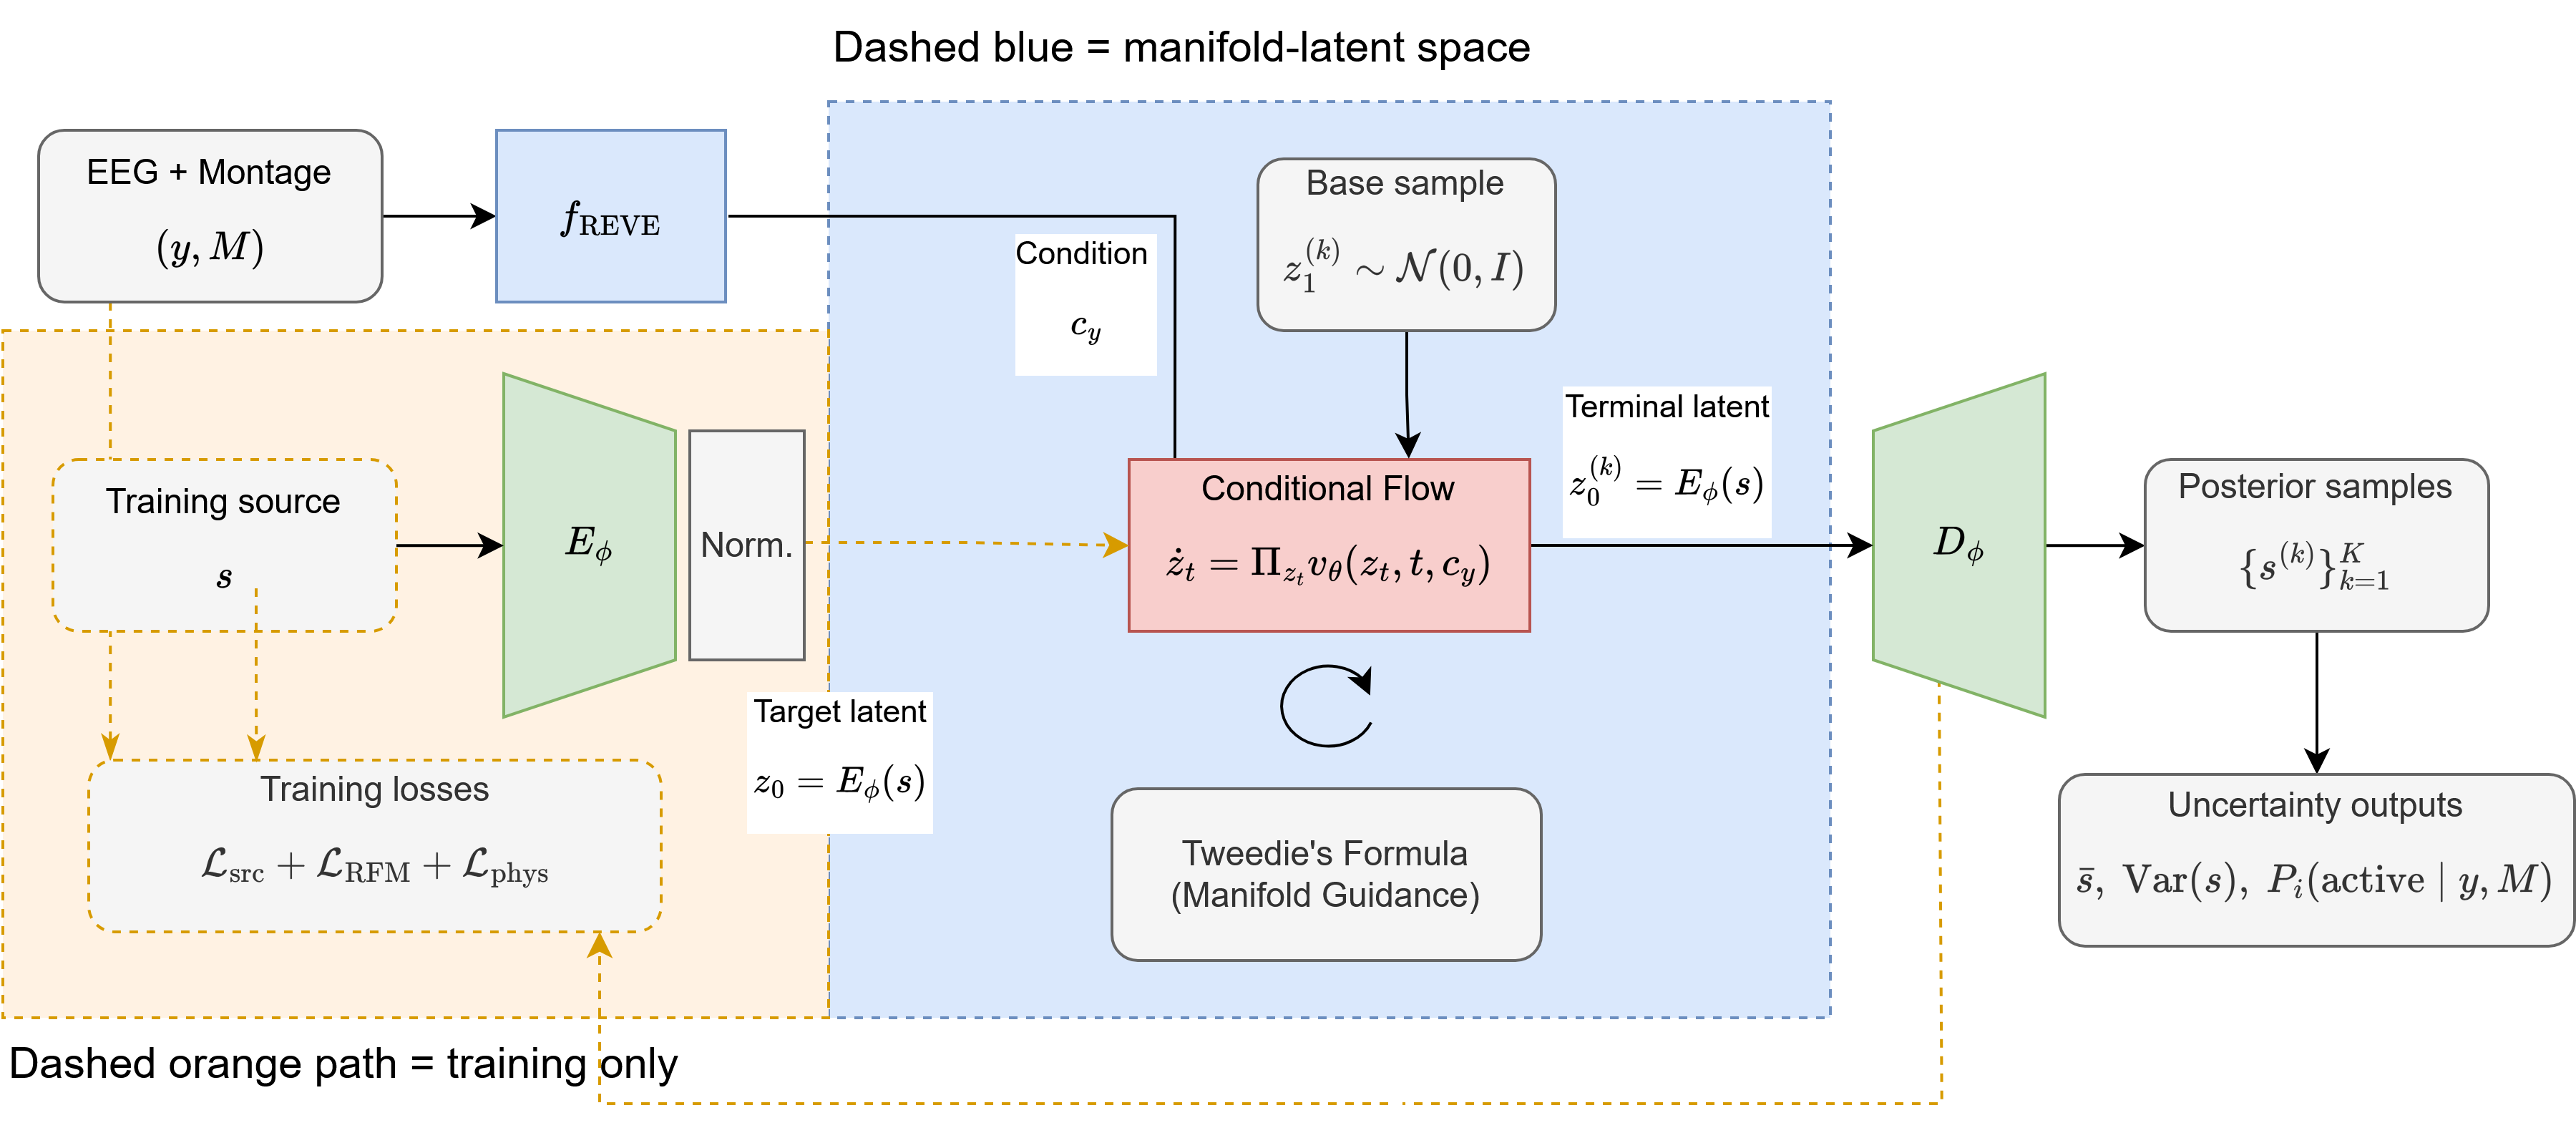
\includegraphics[width=\linewidth]{slide36_architecture.png}
    \end{column}%
    \hfill
    \begin{column}{0.25\textwidth}
      \begin{tikzpicture}[
        every node/.style={font=\scriptsize\sffamily, align=left},
        chip/.style={rounded corners=2mm, line width=0.8pt, inner sep=1.8mm,
                     text width=0.82\linewidth},
      ]
        \node[chip, draw=CERNblue, fill=CERNblue!9] at (0,0)
          {\textbf{Training signal}\\source labels + physics-aware losses};
        \node[chip, draw=CERNorange, fill=CERNorange!10] at (0,-1.45)
          {\textbf{Posterior sampling}\\multiple plausible source maps};
        \node[chip, draw=CERNcyan, fill=CERNcyan!16] at (0,-2.9)
          {\textbf{Outputs}\\mean, variance, active probability};
      \end{tikzpicture}
    \end{column}
  \end{columns}
\end{frame}

%% ===========================================================================
%% Outlook: publication timeline and open question
%% ===========================================================================
\section{Outlook}

\begin{frame}{Publication timeline}
  \centering\footnotesize\color{CERNtextdark}
  Two papers on two tracks, timed around dataset validation.

  \vspace{2mm}
  \begin{tikzpicture}[
    every node/.style={font=\scriptsize\sffamily, align=center},
    stage/.style={rectangle, rounded corners=2mm, very thick,
                  minimum width=34mm, minimum height=18mm,
                  align=center, inner sep=1.5mm},
    arr/.style={-{Stealth[length=2.2mm,width=2mm]}, very thick, CERNblue},
  ]
    \node[stage, draw=CERNblue, fill=CERNblue!15] (p1) at (0,0)
      {{\color{CERNblue}\faFileMedical}\\\textbf{Lorenzo's paper}\\EEG source localization\\\textbf{ICLR}\\mid-September};
    \node[stage, draw=CERNnavy, fill=CERNnavy!12] (val) at (4.6,0)
      {{\color{CERNnavy}\faUserMd}\\\textbf{Dataset validation}\\clinicians finish\\mid-September};
    \node[stage, draw=CERNorange, fill=CERNorange!18] (p2) at (9.2,0)
      {{\color{CERNorange}\faStethoscope}\\\textbf{NeuroAgent paper}\\\textbf{Nature Machine}\\\textbf{Intelligence}\\early October};

    \draw[arr] (p1.east) -- (val.west);
    \draw[arr] (val.east) -- (p2.west);
  \end{tikzpicture}

  \vspace{1.5mm}
  \footnotesize\color{CERNtextdark}
  Work on the Nature Machine Intelligence paper will continue during the summer, ahead of full
  validation, so it is ready to submit within about two weeks of clinician sign-off.

  \vspace{2mm}
  \begin{center}
  \begin{tikzpicture}
    \node[rounded corners=2mm, draw=CERNorange, line width=0.8pt,
          fill=CERNorange!10, inner sep=2.2mm,
          text width=0.9\textwidth, align=center]
    {\footnotesize\color{CERNtextdark}
      {\faQuestionCircle}\;\textbf{Question:} when should I schedule my
      first-year PhD presentation, and what would you recommend given this timeline?};
  \end{tikzpicture}
  \end{center}
\end{frame}

%% ===========================================================================
%% End slide
%% ===========================================================================
\makeend

\end{document}
